\newpage

\chapter{Обработка реального временного ряда с помощью R}

\section{Вычисление основных описательных статистик} % (fold)
\label{sec:dstats}

В качестве исходных данных примем выборку из полученной от учебно-научного центра базы данных, путём отбора наблюдений в июле месяце за период с 1975 по 2012 год. Выборка представлена в приложении А в таблице А.1\todo{Ссылка}. Графически исходные данные представлены на рисунке \ref{img:input}.

\begin{figure}[ht]
\center{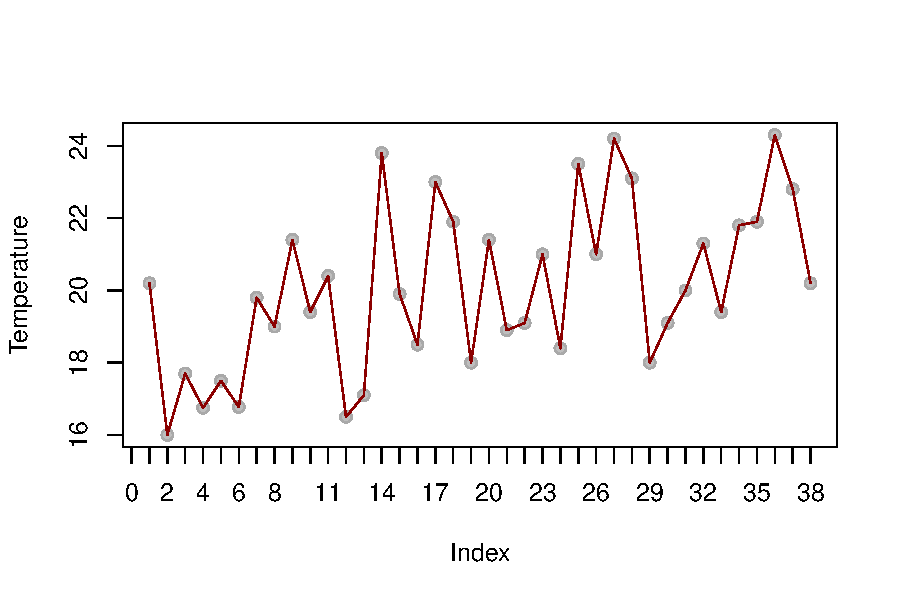
\includegraphics[width=1\linewidth]{../figures/temperature-ts-first-overview.pdf}}
\caption{График исходных данных.}
\label{img:input}
\end{figure}

Начнём исследование временного ряда с вычисления описательных статистик. \textbf{R} предоставляет в пакете \textit{base} такие функции как: \textit{var} --- дисперсия, \textit{mean} --- среднее, \textit{sd} --- стандартное отклонение, \textit{median} --- медиана, \textit{quantile} --- квантили, \textit{range} --- размах, \textit{min, max}. Также, в различных пакетах можно найти другие интерисующие функции, как статистические, так и математические. Но в целях удобства, компактности и контроля за функциональностью мной был написан модуль \textit{dstats}. Данный модуль позволяет вычислять все необходимые в данной работе описательные статистики. 

Для получения всех описательных статистик воспользуемся представленным в [\todo{Ссылка на листинг}] модулем. Полученные результаты представлены в таблице \ref{table:dstats}.


> xtable(dstats, caption="Описательные статистики для наблюдаемых температур", label="table:dstats")
% latex table generated in R 3.0.2 by xtable 1.7-1 package
% Sun Dec  1 02:50:24 2013
\begin{table}[ht]
\centering
\begin{tabular}{rr}
  \hline
 & Значение \\ 
  \hline
Среднее & 20.08 \\ 
  Медиана & 19.95 \\ 
  Нижний квартиль & 18.42 \\ 
  Верхний квартиль & 21.70 \\ 
  Минимум & 16.00 \\ 
  Максимум & 24.30 \\ 
  Размах & 8.30 \\ 
  Квартильный размах & 3.28 \\ 
  Дисперсия & 5.24 \\ 
  Стандартное отклонение & 2.29 \\ 
  Коэффициент вариации & 26.10 \\ 
  Стандартная ошибка & 0.37 \\ 
  Асимметрия & 0.14 \\ 
  Ошибка асимметрии & 0.38 \\ 
  Эксцесс & -0.85 \\ 
  Ошибка эксцесса & 0.75 \\ 
   \hline
\end{tabular}
\caption{Описательные статистики для наблюдаемых температур} 
\label{table:dstats}
\end{table}

> sink()   


Рассмотрим подробнее некоторые полученные статистики.

Как видно из таблицы, \textit{средняя} температура в июле месяце за период с 1975 по 2012 составляет приблизительно 20°С. При этом \textit{размах} температур равен 8.3°C. \textit{Дисперсия} в данном случае равна 5.24.

\textit{Стандартное отклонение} оказалось равным приблизительно $2.3$. Полученное значение не велико, а значит можно сказать, что среднее значение хорошо описывает выборку. И что в среднем, температура воды озера Баторино отличается от полученной ранее \textit{средней} температуры на 2.3°C.

\textit{Коэффициент вариации} в нашем случае равен $26.1\%$. Из этого следует, что выборку можно счиать однородной, так как полученное значение является меньшим 33\%.

\textit{Стандартная ошибка среднего значения} равна $0.37$.

\textit{Коэффициент асимметрии} --- мера симметричности распределения. Полученное значение: $0.14$. Данное значение говорит о незначительном коэффициенте асимметрии выборки. То есть о том, что выборочное распределение можно считать близким к симметричному.

\textit{Cтандартная ошибка асимметрии} равна $0.38$.

\textit{Коэффициент эксцесса} в рассматриваемом случае равен $-0.85$. Так как коэффициент эксцесса нормального распределения равен $0$, то в данном случае можно говорить о пологости пика распределения выборки по отношению к нормальному распределению. 

\textit{Стандартная ошибка коэффициента эксцесса} равна $0.75$. 

По данному ранее определению тестовых статистик для коэффициента асимметрии и эксцесса, проверим значимость полученных значений для генеральной совокупности. Для этого в модуле \textit{dstats} мной реализованы функции \textit{dstats.test.skew} и \textit{dstats.test.kurtosis}:

Полученная тестовая статистика для коэффициента асимметрии:
\begin{equation*}
	Z_{A_S} = \frac{A_S}{SES} = 0.3630143.
\end{equation*}
Данное значение попадает под случай $\vert Z_{A_S} \vert \le 2$, а значит, выборочный коэффициент асимметрии не является значимым. Из чего, в свою очередь, следует, что по нему нельзя судить о коэффициенте асимметрии генеральной совокупности.

Полученная тестовая статистика для коэффициента эксцесса:
\begin{equation*}
	Z_K = \frac{K}{SEK} = -1.135476.
\end{equation*}
Данное значение попадает под случай $\vert Z_K \vert \le 2$, а значит, в данном случае выборочный коэффициент эксцесса не является значимым и нельзя ничего сказать о коэффициенте эксцесса генеральной совокупности.
\todo[inline, color=cyan!60]{Проверить классические тестовые статистики}
\todo[inline, color=purple!70]{Сделать вывод о полученных результатах}
% section dstats (end)

\section{Исследование статистических данных} % (fold)
\label{sec:analysis}

В \textbf{R} можно найти различные пакеты, позволяющие строить разнообразные гистограммы, диаграммы рассеяния, вероятностные графики, линейные графики, диаграммы диапазонов, размахов, круговые диаграммы, столбчатые диаграммы, последовательные графики и т.д., позволяющие увидеть специфику данных.

В пакет \textit{base} для визуализации входят такие функции как:
\begin{itemize}
\item \textit{plot}: общая функция для построения графиков $y(x)$;
\item \textit{barplot}: столбцовые диаграммы;
\item \textit{boxplot}: график ``ящик-с-усами'';
\item \textit{hist}: гистограммы;
\item \textit{pie}: круговые диаграммы;
\item \textit{dotchart}: точечные графики;
\item \textit{image, heatmap, contour, persp}: функции для генерации трёхмерных графиков;
\item \textit{qqnorm, qqline, qqplot}: графики квантилей;
\item \textit{pairs, coplot}: отображают на графиках несколько выборок.
\end{itemize}

С помощью функции \textit{hist} построим гистограмму для отображения вариационного ряда исходных данных. Гистограммы позволяют увидеть, как распределены значения переменных по интервалам группировки, то есть как часто переменные принимают значения из различных интервалов. А также, что бывает более важным, повзоляет сделать предположение о разновидности распределения. Полученная гистограмма отражена на рисунке \ref{img:histogram}. 
\begin{figure}[ht]
\center{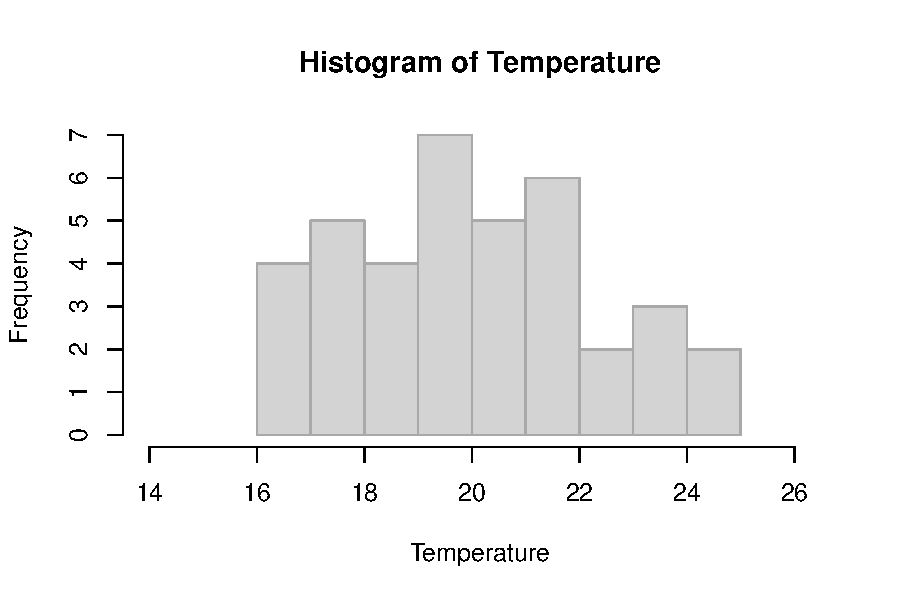
\includegraphics[width=1\linewidth]{../figures/temperature-histogram.pdf}}
\caption{Гистограмма наблюдаемых температур.}
\label{img:histogram}
\end{figure}

Представленная гистограмма построена с автоматически рассчитанным количеством интервалов разбиения. Воспользуемся \textit{формулой Стерджеса} для вычисления этого количества. Из [\todo{Sturges}] количество интервалов разбиения рассчитывается по формуле:
\begin{equation}
\label{eq:sturges}
	k = \lceil log_{2}n \rceil + 1 = \lceil log_{2}38 \rceil + 1 = 7.
\end{equation}
Следует отметить, что в построенной гистограмме, на рисунке \ref{img:histogram}, получилось 9 интервалов. Данный результат обосновывается особенностями реализации функции \textit{hist}. Указанная особенность заключается в том, что эта функция вычисляет количество интервалов по формуле Стерджеса \ref{eq:sturges} и при построении интервалов пользуется принципом ``красивого'' разбиения\todo{не очень хорошее объяснение}.

По полученной гистограмме можно визуально предположить близость выборочного распределения к нормальному распределению. Исследуем подробнее данное наблюдение.

Для этого построим гистограмму с кривой плотности нормального распределения. Построенная гистограмма отображена на рисунке \ref{img:histogram_fitted}.
\begin{figure}[ht]
\center{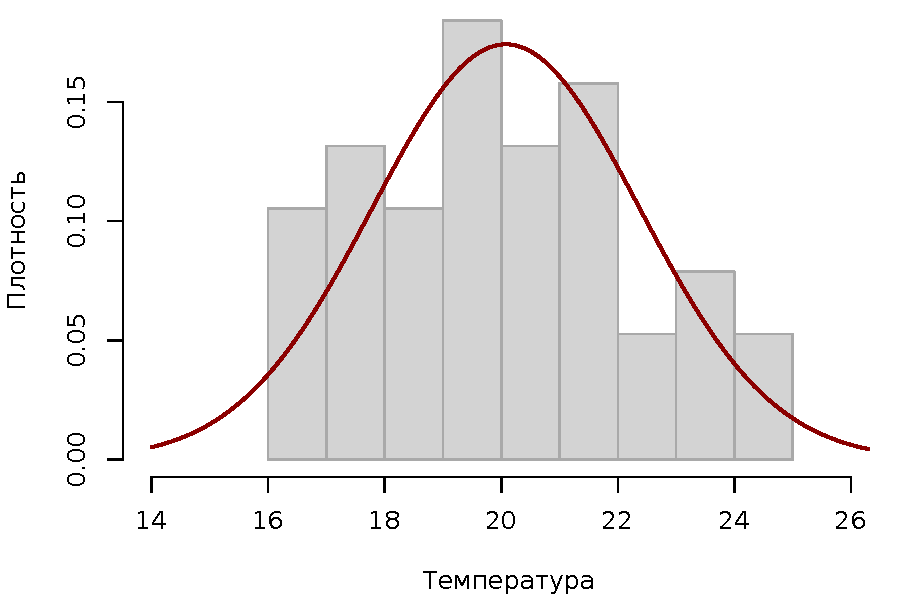
\includegraphics[width=1\linewidth]{../figures/temperature-histogram-dnorm.pdf}}
\caption{Гистограмма наблюдаемых температур с кривой плотности нормального распределения.}
\label{img:histogram_fitted}
\end{figure}
На основании этой диаграммы уже можно сказать больше. Во-первых, здесь нагляднее представлена близость выборочного распределения к нормальному. Во-вторых, по этой гистограмме можно подтвердить или опровергнуть результаты, полученные на этапе вычисления описательных статистик в параграфе \ref{sec:dstats}.

Следует отметить согласованность полученных описательных статистик с полученной гистограммой. Во-первых, по коэффициенту асимметрии мы предположили о близости распределения к симметричному. Это подтверждается гистограммой: на ней можно заметить небольшую скошенность вправо, что также согласовывается со знаком коэффициента. Во-вторых, коэффициент эксцесса указывал на пологость пика распределения. Данное заключение подтверждается кривой плотности --- она имеет чуть более растянутую колоколобразную форму.

Другим очень часто используемым графическим способом проверки характера распределения данных является построение т.н. \textit{графиков квантилей} (\textit{Q-Q plots}, \textit{Quantile-Quantile plots}). На таких графиках изображаются квантили двух распределений --- эмпирического (т.е. построенного по анализируемым данным) и теоретически ожидаемого стандартного нормального распределения. При нормальном распределении проверяемой переменной точки на графике квантилей должны выстраиваться в прямую линию, исходящую под улом 45 градусов из левого нижнего угла графика. Графики квантилей особенно полезны при работе с небольшими по размеру совокупностями, для которых невозможно построить гистограммы, принимающие какую-либо выраженную форму.

В \textbf{R} для построения графиков квантилей можно использовать базовую функцию \textit{qqnorm} (Рисунок \ref{img:qqnorm})
\begin{figure}[ht]
\center{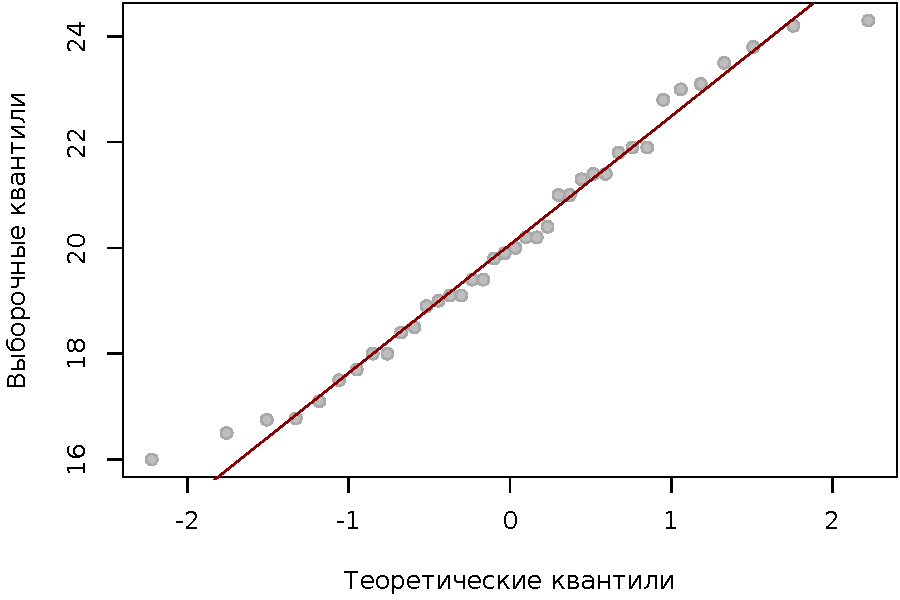
\includegraphics[width=1\linewidth]{../figures/temperature-qqnorm.pdf}}
\caption{График квантилей для наблюдаемых температур.}
\label{img:qqnorm}
\end{figure}
На этом графике можно визуально обнаружить аномальное положение наблюдаемых значений по отношению к нормальному распределению. В данном случае отклонения можно наблюдать на концах рассматриваемого промежутка. Остальные значения образуют отчетливую прямую. А значит, подтверждается предположение о нормальности выборочного распределения.

Далее следует проверить полученные результаты с помощью некоторых формальных тестов. Существует целый ряд статистических тестов, специально разработанных для проверки нормальности выборочного распределения. В общем виде проверяемую при помощи этих тестов нулевую гипотезу можно сформулиировать следующим образом: ``Анализируемая выборка происходит из генеральной совокупности, имеющей нормальное распределение''. Если получаемая при помощи того или иного теста вероятность ошибки $P$ оказывается меньше некоторого заранее принятого уровня значимости (например, $0.05$), нулевая гипотеза отклоняется.

В \textbf{R} реализованы практически все имеющиеся тесты на нормальность --- либо в виде стандарных функций, либо в виде функций, входящих в состав отдельных пакетов. Примером базовой функции является \textit{shapiro.test()}, при помощи которой можно выполнить широко используемый \textit{тест Шапиро-Уилка}:
\begin{verbatim} 

	Shapiro-Wilk normality test

data:  Temperature
W = 0.9742, p-value = 0.5685

\end{verbatim}
В полученных результатах $W$ --- статистика Шапиро-Уилка. Вероятность ошибки $p = 0.4706 > 0.05$, а значит нулевая гипотеза не отвергается. Следовательно опровергнуть предположение на основе данного теста нельзя.

Попробуем опровегнуть наше предположение на основе проверки критерия $\chi^2$ Пирсона. Для этого воспользуемся пакетом \textit{nortest} и функцией \textit{pearson.test}:
\begin{verbatim} 

	Pearson chi-square normality test

data:  Temperature
P = 2.8, p-value = 0.8335

\end{verbatim}
В полученных результатах $P$ --- статистика $\chi^2$ Пирсона. Вероятность ошибки $p = 0.938 > 0.05$, а значит нулевая гипотеза не отвергается. Следовательно опровергнуть предположение о нормальности на основе данного теста также нельзя. Проверим критерий: примем уровень значимости $\alpha = 0.05$, тогда из таблицы распределения $\chi^2$ найдём критическое значение критерия $\chi_{\textrm{кр}}^2(\alpha, k) = 7.8$. Отсюда следует, что

\begin{equation*}
	\chi_{\textrm{набл}}^2 < \chi_{\textrm{кр}}^2,
\end{equation*}
где $\chi_{\textrm{набл}}^2 = P = 1.7895$.

А значит, нулевую гипотезу при уровне значимости $\alpha = 0.05$ не отвергаем и подтверждаем сделанный вывод на основании вычисленной вероятности ошибки. 

Воспользуемся для тех же целей критерием Колмогорова--Смирнова. Как в предыдущем случае воспользуемся представленной в пакете \textit{nortest} функцией \textit{ks.test}:
\begin{verbatim} 

	Two-sample Kolmogorov-Smirnov test

data:  Temperature and test.nsample
D = 0.0661, p-value = 0.9964
alternative hypothesis: two-sided

\end{verbatim}
Вероятность ошибки $p > 0.05$, а значит нулевую гипотезу отвергнуть нельзя. Следовательно опровергнуть предположение о нормальности, как и предыдущих случаях, также нельзя. Проверим критерий: примем так же уровень значимости $\alpha = 0.05$, тогда критическое значение $D_{\textrm{кр}}(\alpha) = 1.358$. Следовательно,
\begin{equation*}
	D < D_{\textrm{кр}}(\alpha),
\end{equation*}
и подтверждаем сделанные ранее заключения: нельзя отвергнуть нулевую гипотезу о нормальности выборочного распределения.

В соответствии с результатами проверки критериев и на основе построенных гистограммы и графика квантилей, можно сделать заключение о том, что распределение температуры воды озера Баторино в июле 1975--2012 годов является близким к нормальному закону распределения.

Воспользуемся ещё одним из графических инструментов анализа данных --- Bag Plot (диаграмма концентрации). 
Диаграмма концентрации является двумерным обобщением широко известного графика <<ящик-с-усами>>. Данный инструмент применяется для поиска нетипичных наблюдений по сочетанию пары количественных признаков (в нашем случае это дата и температура). Основными компонентами данной диаграммы являются <<мешок>>, который 
содержит $50\%$ значений выборки, граница, которая отделяет внутренние точки от выбросов, и контур, показывающий точки снаружи «мешка», но внутри границы. Аналогично диаграмме размаха, диаграмма концентрации 
визуализирует некоторые характеристики выборочных данных: положение выборки (расположением медианы), распространение (размер «мешка»), корреляция (ориентация «мешка»), асимметрия (форма «мешка» и контура), 
хвосты (точки на границе контура и выбросы)[\todo{Ссылка}].

Результат построения диаграммы проиллюстрирован на рисунке \ref{img:bagplot}.
\begin{figure}[ht]
\center{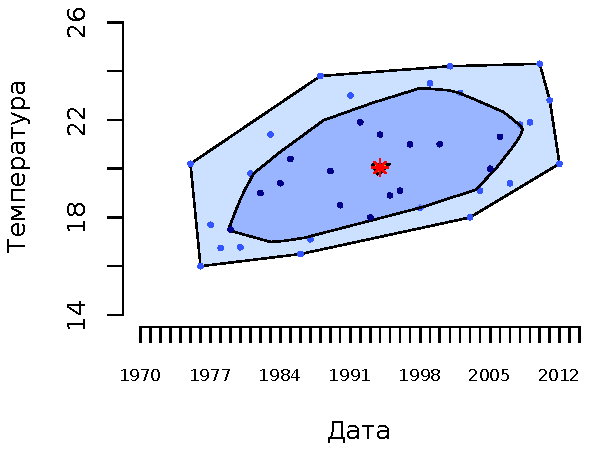
\includegraphics[width=1\linewidth]{../figures/bagplot.pdf}}
\caption{Диаграмма концентрации.}
\label{img:bagplot}
\end{figure}
В центре полученной диаграммы находится медиана, <<мешок>> обозначен темным оттенком, контур светлым, выбросы обозначены перекрестием. Следовательно, выбросы не обнаружены, но следует отметить, что несколько точек находятся на самой границе контура --- будем считать их подозрительными на выброс. По диаграмме также можно сказать о корреляции рассматриваемых переменных: <<мешок>> ориентирован вверх, что говорит о положительной корреляции. Также можно сделать заключения по асимметрии и проверить результаты, полученные на этапе вычисления описательных статистик. На диаграмме можно видеть, полученная фигура очень похожа на эллипс с центром, обозначенным медианой. Как следствие этого, можно судить о близости выборочного распределения с симметричным распределением, что подтверждает полученные ранее в анализе описательных статистик, представленных в таблице \ref{table:dstats}, результаты.

На данном этапе по результатам полученных на основе графиков \ref{img:qqnorm} и \ref{img:bagplot} возникли подозрения о выбросах в исходной выборке. Выявление таких аномальных значений важно, так как их наличие, как правило, сильно влияет на всю выборку, в частности, на коэффициент корреляции. Проверим наличие выбросов с помощью статистических критериев. Для этих целей воспользуемся критерием Граббса. Воспользуемся им для определения наличия выбросов в исходной выборке. 

Полученные результаты проверки критерия Граббса:
\begin{verbatim} 

	Grubbs test for one outlier

data:  Temperature
G = 1.9487, U = 0.8850, p-value = 0.8103
alternative hypothesis: highest value 24.2 is an outlier

\end{verbatim}
Данный результат ($p$-value$ = 1$) однозначно говорит нам о том, что следует отклонить альтернативную гипотезу $H_{1}$ и принять гипотезу $H_{0}$. Другими словами, это говорит о том, что в исходной выборке нету выбросов. А значит выборка однородна. Значит, наши предположения о выбросах на основе графического представления выборки оказались не подтвердились проверкой критерия\todo[size=\tiny]{+cite: Grubbs, F.E. (1950). Sample Criteria for testing outlying observations. Ann. Math. Stat. 21, 1, 27-58.}.

Исследуем теперь зависимость температуры воды от времени, построив диаграмму рассеяния и вычислив коэффициент соответствующих переменных.

Для начала построим корреляционную матрицу.
% latex table generated in R 3.0.1 by xtable 1.7-1 package
% Tue Dec  3 12:51:29 2013
\begin{table}[ht]
\centering
\begin{tabular}{rrr}
  \hline
 & Temperature & Date \\ 
  \hline
Temperature & 1.00 & 0.52 \\ 
  Date & 0.52 & 1.00 \\ 
   \hline
\end{tabular}
\caption{Корреляционная матрица.} 
\label{table:cmatrix}
\end{table}

Как видно из таблицы \ref{table:cmatrix}, коэффициент корреляции $r_{xt}=0.52$. Этим подтверждается наши выводы из диаграммы концентрации о положительной корреляции, поскольку полученный коэффициент корреляции является положительным по характеру и по таблице \ref{table:corr} средним (умеренным) по силе: $0.5 < r_{xt} < 0.7$.

Попробуем оценить значимость полученного выборочного коэффициента корреляции с помощью возможностей пакета \textbf{R} и описанного ранее критерия значимости\todo{Может стоит сделать нумерацию для критерия, чтобы делать на него ссылку?}.

Пакет \textbf{R} предоставляет с помощью функции \textit{cor.test} различные методы для проверки значимости выборочного коэффициента корреляции. Воспользуемся проверкой теста методом Пирсона:
\begin{verbatim} 

	Pearson's product-moment correlation

data:  Temperature and Date
t = 3.6801, df = 36, p-value = 0.0007579
alternative hypothesis: true correlation is not equal to 0
95 percent confidence interval:
 0.2439316 0.7218701
sample estimates:
      cor 
0.5228432 

\end{verbatim}
Как видно из полученных результатов $p-value < 0.05$, следовательно это говорит о том, что необходимо отвергнуть нулевую гипотезу.

Проверим с помощью критерия:
\begin{equation*}
	T_{\textrm{набл}} = \frac{r_{xt} \sqrt{n - 2}}{\sqrt{1 - r_{xt}^2}} \approx 3.98095.
\end{equation*}
Примем уровень значимости $\alpha = 0.05$. Число степеней свободы $k = n - 2 = 36$ (что подтверждает вычисленное функцией значение \textit{df}). Тогда из таблицы критических точек распределения Стьюдента $t_k \approx 2,03$. Следовательно,
\begin{equation*}
	T_{\textrm{набл}} > t_k	
\end{equation*}
Значит, нулевую гипотезу отвергаем и подтверждаем правильность полученных с помощью \textbf{R} результатов. Другими словами, выборочный коэффициент значимо отличается от нуля, т.е. температура воды и время при уровне значимости $\alpha = 0,05$ имеют зависимость.

Проиллюстрируем предположенную зависимость с помощью двумерной диаграммы рассеяния. Данные диаграммы используются для визуального исследования зависимости между двумя переменными. Если переменные сильно связаны, то множество точек данных принимает определённую форму. С помощью таких диаграмм можно наглядно изучить знак коэффициента корреляции. Если точки на диаграмме расположены хаотически, то это говорит о независимости рассматриваемых переменных. Если с ростом переменной $t$ возрастает переменная $x$ то имеет место положительная корреляция. Если же с ростом переменной $t$ переменная $x$ убывает, то это указывает на отрицательную корреляцию. Построим такую диаграмму и проверим полученные ранее результаты в таблице \ref{table:cmatrix}.
\begin{figure}[ht]
\center{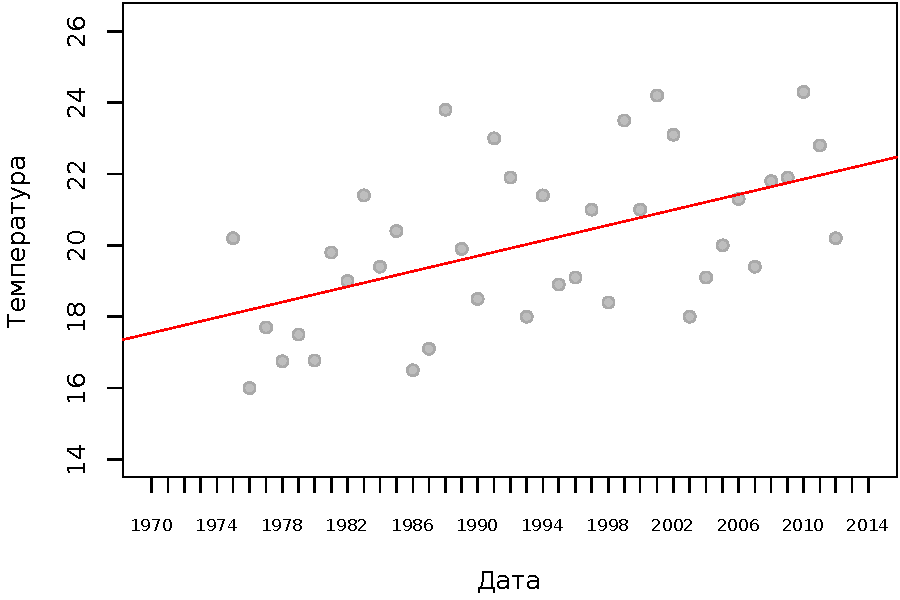
\includegraphics[width=1\linewidth]{../figures/scatterplot.pdf}}
\caption{Диаграмма рассеяния.}
\label{img:scatterplot}
\end{figure}

Из рисунка \ref{img:scatterplot} видно, что точки образуют своеобразное <<облако>>, ориентированное по диагонали вверх. Что, в свою очередь, подтверждает полученные ранее результаты о коррелированности температуры и времени, в том числе и положительность коэффициента корреляции (ориентированность вверх). Но при этом, данная диаграмма наглядно показывает степень коррелированности: так как точки не образуют чёткой формы, а разбросаны относительно диагонали, то можно говорить о наличии умеренной корреляции. То есть, нельзя сказать, что корреляция сильная, но и нельзя сказать, что связь между переменными отсутствует.
\todo[inline, color=purple!70]{Думаю, здесь нужно сделать выводы о проделанной в данной части работе --- подвести итог}
% section analysis (end)